\documentclass[aspectratio=169,obeyspaces,spaces,hyphens,dvipsnames]{beamer}
\usepackage[utf8]{inputenc}
\usepackage{minted}
\usepackage{hyperref}

\mode<presentation>
\usetheme{FreeElectrons}

\def\signed #1{{\leavevmode\unskip\nobreak\hfil\penalty50\hskip2em
  \hbox{}\nobreak\hfil(#1)%
  \parfillskip=0pt \finalhyphendemerits=0 \endgraf}}

\newsavebox\mybox
\newenvironment{aquote}[1]
  {\savebox\mybox{#1}\begin{quotation}}
  {\signed{\usebox\mybox}\end{quotation}}

\title{Running UBI/UBIFS on MLC NAND}
\conference{Embedded Linux Conference 2016}
\authors{Boris Brezillon, Richard Weinberger}
\email{boris@free-electrons.com, richard@sigma-star.at}
\institute{Free Electrons, sigma star gmbh}
\slidesurl{http://free-electrons.com/pub/conferences/2016/elc/brezillon-nand-framework}

\begin{document}

\addtocontents{toc}{\protect\setcounter{tocdepth}{-1}}
\section{Running UBI/UBIFS on MLC NAND}
\addtocontents{toc}{\protect\setcounter{tocdepth}{2}}

\subsection{MLC NANDs constraints: where the nightmare begins}

\begin{frame}{SLC NANDs: Boring, our happy place}
  \begin{figure}
  \includegraphics[scale=0.05]{Macaca_fuscata_juvenile_yawning.jpg}
   \end{figure}
% or maybe this one? https://en.wikipedia.org/wiki/Wikipedia:Featured_picture_candidates/Japanese_macaque_juvenile_yawning
\end{frame}

\begin{frame}{MLC NANDs: A nightmare}
  \begin{figure}
  
\includegraphics[scale=0.1]{hand-984170_1920.jpg}
   \end{figure}
% https://pixabay.com/de/hand-silhouette-form-horror-984170/
\end{frame}

\begin{frame}{MLC NAND constraints: What we knew}
  \begin{itemize}
  \item Reduced lifetime: limited number of P/E cycles (5000-10000).
  \item Pages within an erase block have to be programmed in ascending
	order.
  \item Data rentention issues: pretty much the same problem we see
	on SLC NANDs, but a different order of magnitude.
  \item Paired pages: why the hell did they decide to assign the same
	cell to different NAND pages?
  \item Unstable bits: you'd better make sure your board has enough
	power to finish the current erase or program operation, and
	prevent future operations from happening when you are about to
	experience a power-cut.
  \end{itemize}
\end{frame}

\begin{frame}{MLC NAND constraints: Reduced lifetime}
  \begin{itemize}
  \item Not a big problem: we just need to make sure we correctly
	distribute the wear over the NAND device.
  \item UBI is already taking care of that.
  \item May require some tweaking at the UBI level: the default values
	are not suitable for MLC NANDs.
  \end{itemize}
\end{frame}

\begin{frame}{MLC NAND constraints: Data retention issues (1)}
  \begin{itemize}
  \item A NAND cell can see its state changed (charge loss or gain):
	this is what we call bitflips.
  \item Two known sources:
    \begin{itemize}
    \item Read/write disturbance: reading/programming a cell can
	  change neighbour cells state
    \item Inherent charge loss: NAND cells tend to loose their
	  charge over-time. This is emphasized when NAND cells are
	  worn out.
    \end{itemize}
  \item Solutions:
    \begin{itemize}
    \item Increase the ECC strength: usually, this is NAND controller
	  dependent, and even with a strong ECC, you'll hit
	  uncorrectable errors at some point.
    \item Regularly read NAND eraseblocks to detect those that are
	  showing a lot of bitflips, and move the data somewhere else
	  before the ECC is unable to correct these errors.
    \end{itemize}
  \end{itemize}
\end{frame}

\begin{frame}{MLC NAND constraints: Data retention issues (2)}
  \begin{itemize}
  \item MLC cells expose 4 different states instead of 2 states for
	SLC cells.
  \item In MLC cells, distances between states are smaller: data
	retention issues are emphasized.
  \item The smaller the process the closer the cells are, which makes
	read/write disturbance worse.
  \end{itemize}
\end{frame}

\begin{frame}{MLC NAND constraints: Unstable bits}
  \begin{itemize}
  \item Problem described here
	\url{http://www.linux-mtd.infradead.org/doc/ubifs.html\#L_unstable_bits}
  \item Reported by some people on the MTD mailing list
  \item We did not see it during our experimentation
  \item NAND vendors do not communicate on this problem and each
	time we ask, they say they are not aware of this kind of
	problems.
  \item What is described as a black and white problem may actually
	be more subtle: interrupting a program or erase operation
	just before it finishes might leave the page/block in a 'valid'
	state but with a lot of bitflips.
  \item If this assumption turns out to be true, UBI should be able to
	detect that the number of bitflips is high and decide to move
	the data somewhere else or re-erase the block.
  \end{itemize}
\end{frame}

\begin{frame}{MLC NAND constraints: MLC cells}
  \begin{center}
    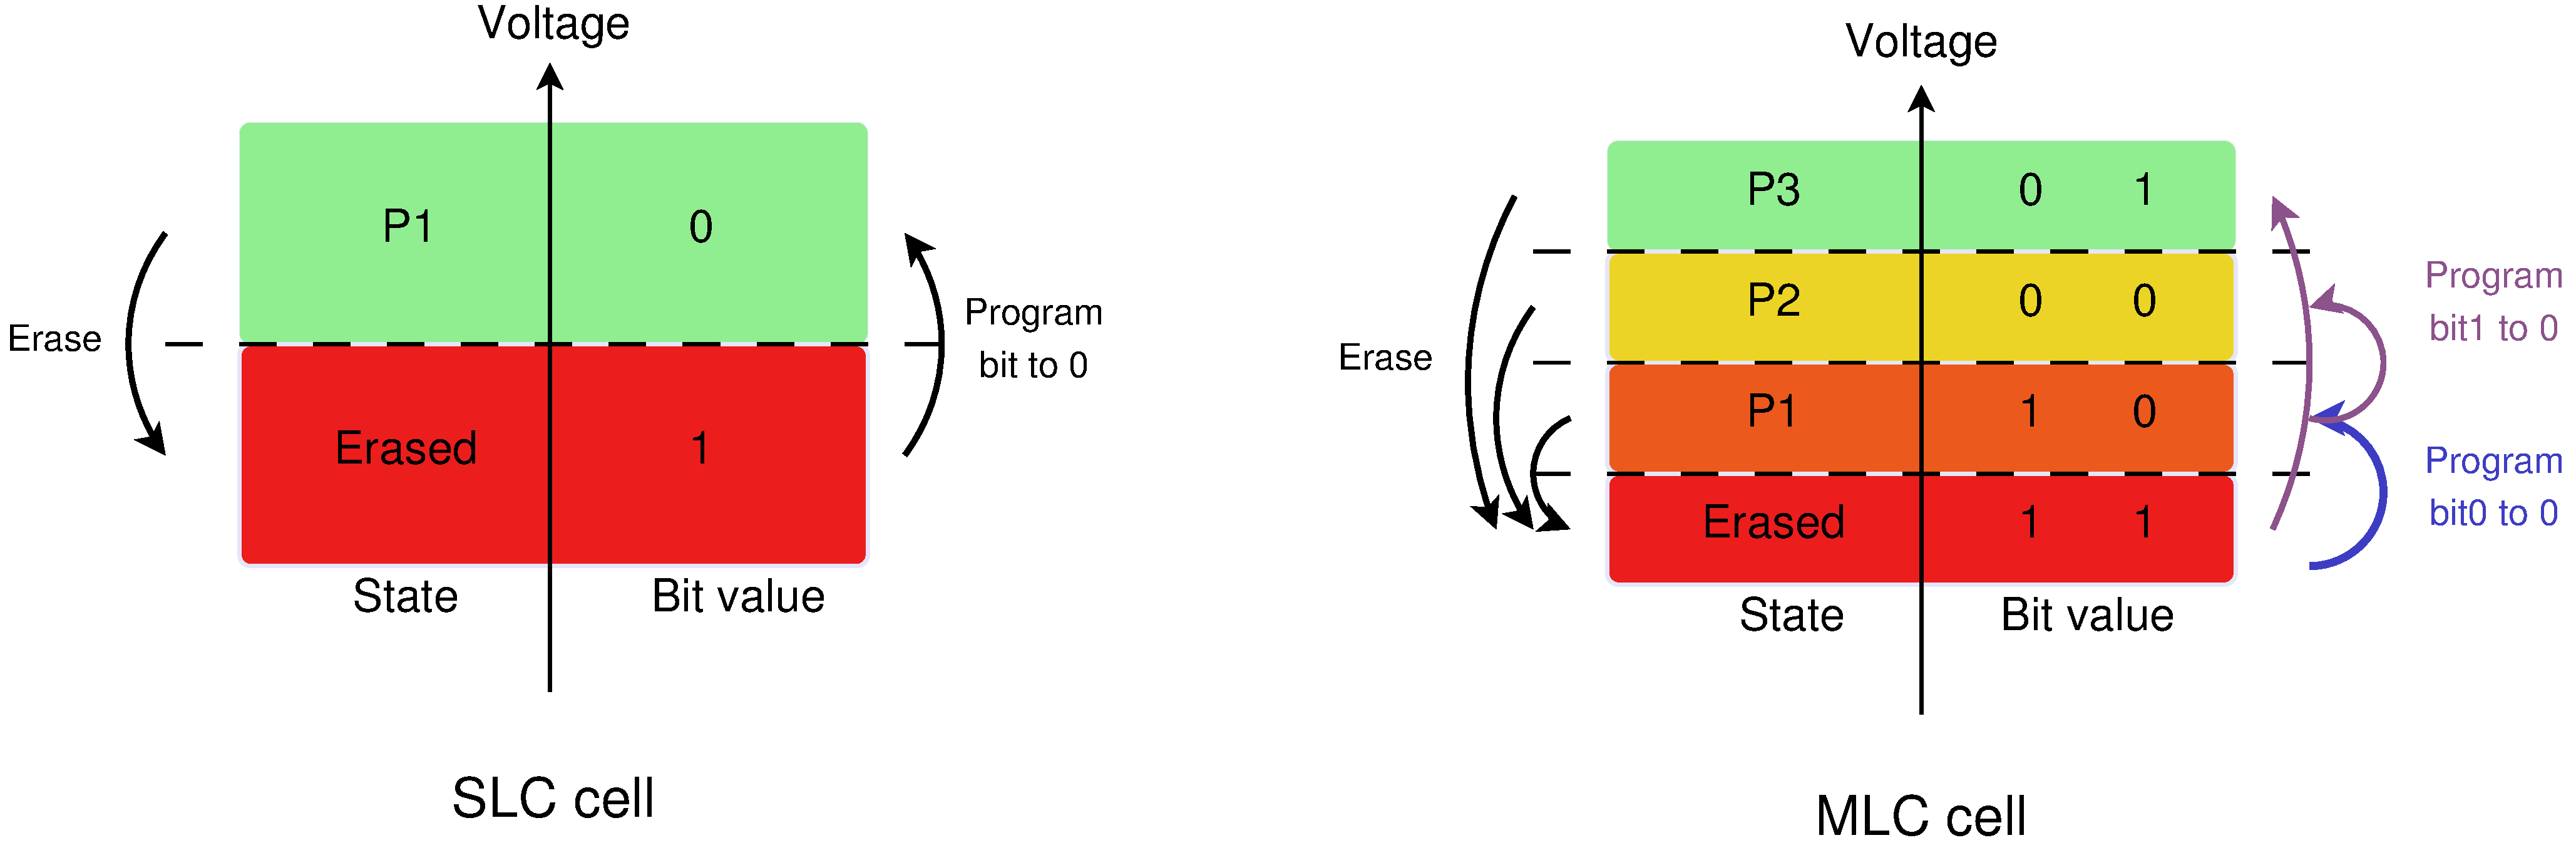
\includegraphics[scale=0.2]{slc-mlc-cell.pdf}
  \end{center}
\end{frame}

\begin{frame}{MLC NAND constraints: Paired pages}
  \begin{itemize}
  \item This is one of the biggest problem we have with MLC NANDs.
  \item MLC cells expose two bits.
  \item Each bit is assigned to a different page.
  \item Pages sharing the same cells are called "Paired pages".
  \item Paired pages are usually not contiguous.
  \item Pages have to be programmed in order.
  \item When programming the second page of a pair, you may corrupt
	the first page of the pair if the operation is interrupted.
  \end{itemize}
\end{frame}

\begin{frame}{MLC NAND constraints: Paired pages}
  \begin{center}
    \includegraphics[scale=0.5]{pairing-scheme.pdf}
  \end{center}
\end{frame}

\begin{frame}{MLC NAND constraints: What we discovered (bad news)}
  \begin{itemize}
  \item Modern MLC NANDs require data scrambling.
  \item Modern MLC NANDs show a high number of bitflips in the last
	set of programmed pages if the erase block is partially
	written.
  \item Both aspects seem to be related:
    \begin{itemize}
    \item NAND vendors try to mitigate the write-disturb effect by
	  accounting for future write-disturb when programming a page.
    \item These write-disturb prediction models are assuming random
	  data, hence the need for data scrambling/randomization.
    \end{itemize}
  \item Let's call this problem the 'Open block' issue.
  \end{itemize}
\end{frame}

\begin{frame}{MLC NAND constraints: What we discovered (good news)}
  \begin{itemize}
  \item MLC NANDs can be programmed in 'SLC mode' (only write the first
	page of each pair)
    \begin{itemize}
    \item This solves the paired pages problem.
    \item Erase blocks written in 'SLC mode' show less bitflips.
    \item Erase blocks written in 'SLC mode' are less sensitive to
	  read/write disturbance.
    \end{itemize}
  \item To summarize, 'SLC mode' makes MLC NAND usable.
  \item But this also means exposing half the storage capacity.
  \end{itemize}
\end{frame}

\begin{frame}{MLC NAND constraints: What we discovered}
  \begin{itemize}
  \item It's a shame we had discover those problems while developing the
	solution.
  \item More details from NAND vendors would be great.
  \item Yes, I'm looking at you, Hynix, Toshiba, Micron, \ldots
  \end{itemize}
\end{frame}

\subsection{UBI: A quick reminder}

\begin{frame}[fragile]
\frametitle{First some basics: UBI nomenclature}
  \begin{itemize}
  \item[PEB] Physical erase block.
  \item[LEB] Logical erase block.
  \item[Image] UBI on your MTD partition.
  \item[Device] Runtime representation of your UBI image (i.e. \textbf{/dev/ubi0}).
  \item[Volume] A volume within the UBI image (i.e. \textbf{/dev/ubi0\_0}).
  \item[Attach] Process of loading an UBI image (i.e. attach mtd0).
  \end{itemize}
\end{frame}

\begin{frame}[fragile]
\frametitle{UBI example}
  \begin{figure}
    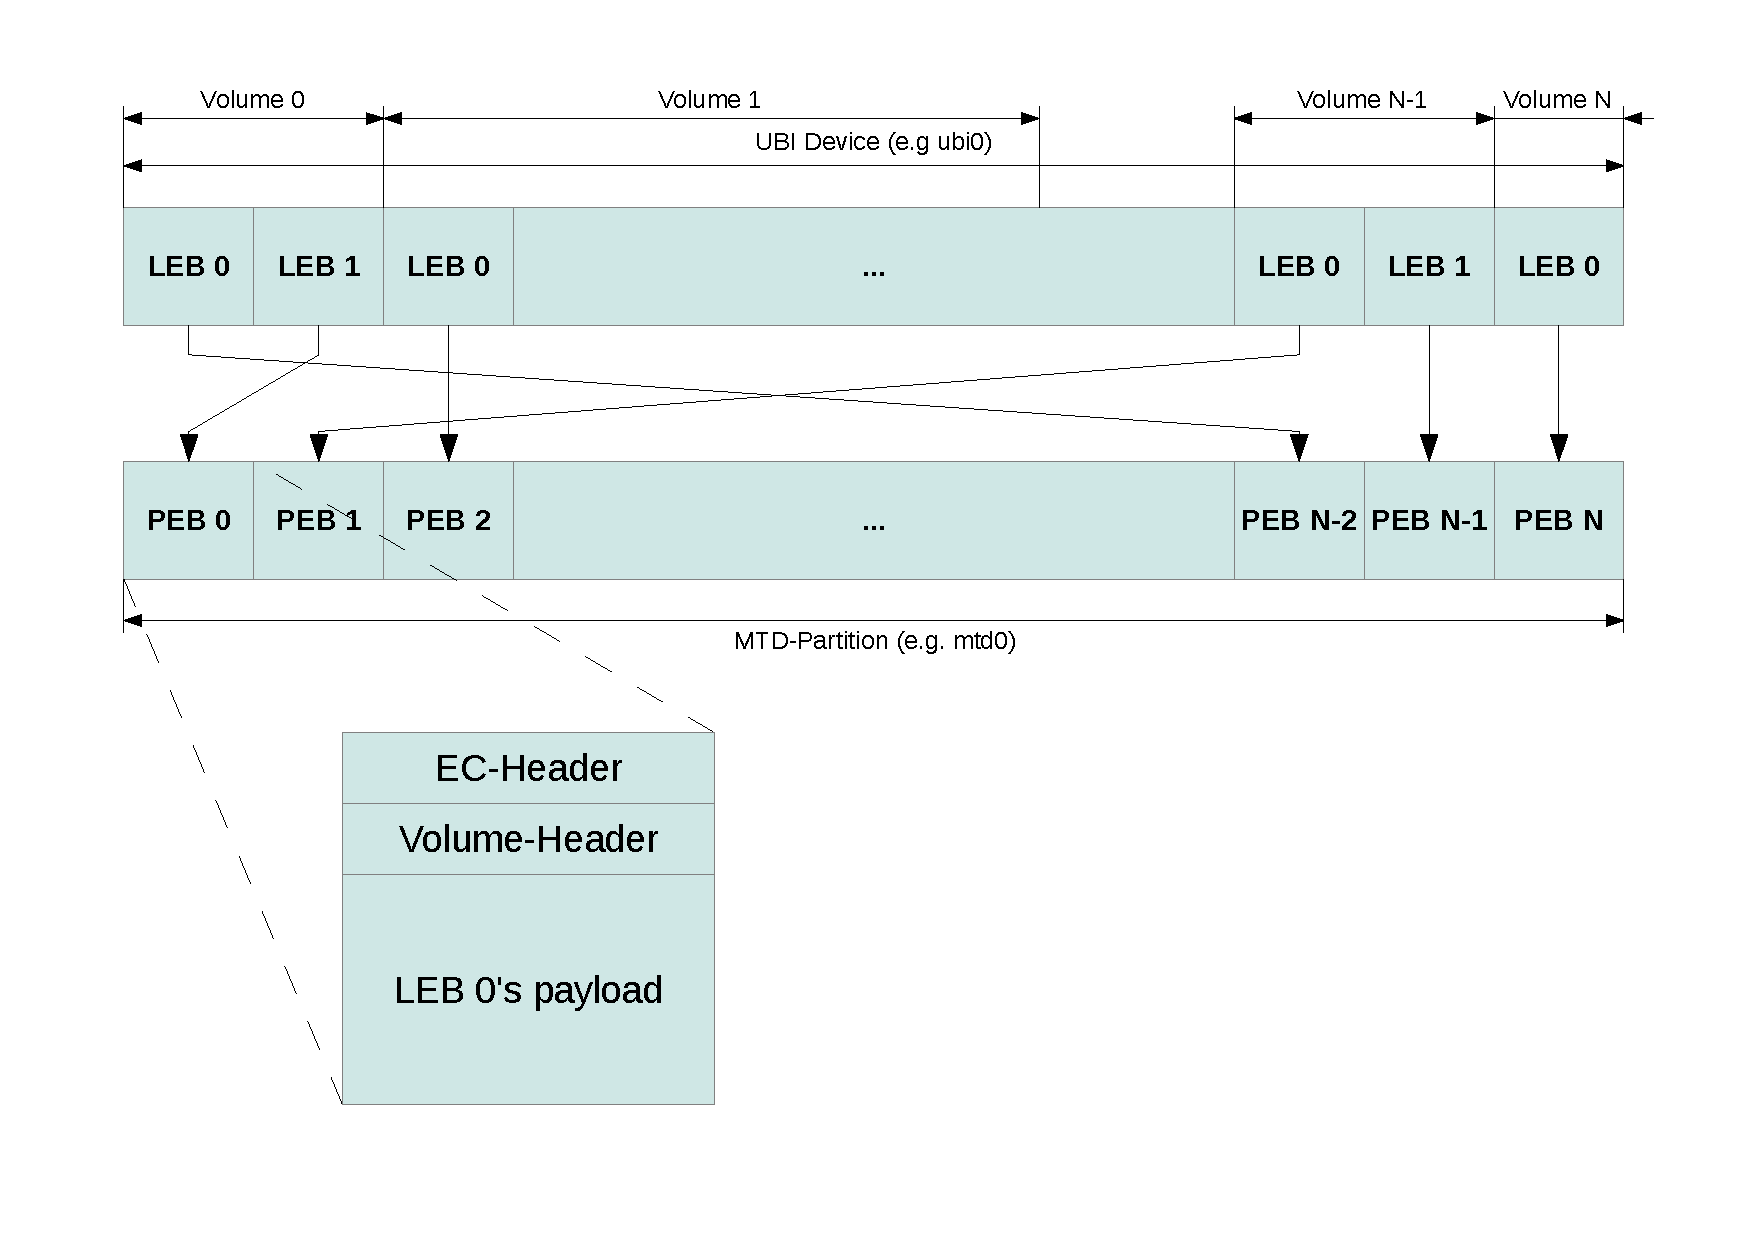
\includegraphics[scale=0.33]{ubi-nonfastmap.pdf}
  \end{figure}
\end{frame}

\begin{frame}[fragile]
\frametitle{UBI PEB on SLC NAND}
   \begin{columns}
   \column{0.5\textwidth}
     \begin{figure}
     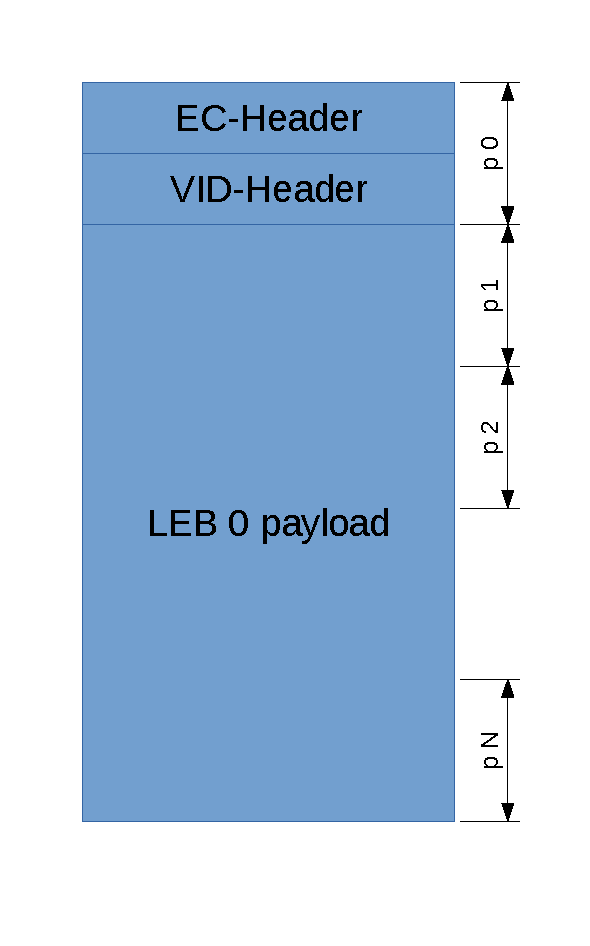
\includegraphics[scale=0.40]{ubi_slc.pdf}
     \end{figure}
   \column{0.5\textwidth}
    \begin{itemize}
    \item Erase count and volume ID header are located on the first page.
    \item If subpages are not supported, volume ID header will be placed on the second page.
    \item Other pages are used for payload.
    \end{itemize}
   \end{columns}
\end{frame}

\subsection{Addressing the data retention issue}

\begin{frame}{Dealing with read disturb}
  \begin{itemize}
  \item On MLC read disturb is a serious problem.
  \item Reading back all data from time to time is needed to detect bitflips.
  \item ubihealthd queries read counters from userspace and trigger reads.
  \item It does not trigger bulk reads such that other applications are not
	impacted.
  \end{itemize}
\end{frame}

\subsection{Addressing the paired pages issue}

\begin{frame}{Expose page pairing schemes}
  \begin{itemize}
  \item Various page pairing scheme found in the wild.
  \item Most pairing schemes follow a predictable logic.
  \item Can be described without a full association table.
  \item New interface to describe these pairing schemes.
  \item The NAND framework will provide an implementation for each pairing scheme.
  \item Pairing scheme selection should be based on NAND detection information.
  \item MTD provides a API to let MTD users query pairing information.
  \end{itemize}
\end{frame}

\begin{frame}{Handle the problem in UBIFS (our first attempts)}
  \begin{itemize}
  \item Proposals:
    \begin{itemize}
    \item 1) Write everything in 'SLC mode' and consolidate UBIFS nodes in MLC
	  mode when we are running out of space.
    \item 2) Write everything in 'MLC mode' (except critical data) and skip
	    pages when we need to secure data (at sync/commit time).
    \end{itemize}
  \item Pros:
    \begin{itemize}
    \item UBIFS knows exactly which data are valid and dirty.
    \item UBIFS knows when data protection is required (i.e. at sync and commit
	  time).
    \end{itemize}
  \item Cons:
    \begin{itemize}
    \item Solution 2 is not possible because of the convoluted pairing schemes
	  and the 'open block' issue.
    \item Solution 1 is too invasive (requires exposing two modes with different
	  LEB size).
    \end{itemize}
  \end{itemize}
\end{frame}

\begin{frame}{Handle the problem in UBI}
  \begin{itemize}
  \item By default every LEB is written in 'SLC mode'.
  \item Obviously we'd waste half the storage capacity.
  \item As soon we run out of available free space, UBI will consolidate
	two fully written SLC LEBs into one MLC PEB and we gain one more LEB
	which can be written again in 'SLC mode'.
  \item That way we can utilize all pages.
  \item Sounds pretty easy, right?
  \end{itemize}
\end{frame}

\begin{frame}{LEB consolidation: when does it take place?}
  \begin{itemize}
  \item As soon as all low pages of a PEB are written the corresponding LEB is
	considered full and becomes a candidate for consolidation.
  \item Bonus question: Why has it to be full?
  \item To produce one free PEB, UBI selects two PEBs that host full LEBs,
	copies their data into a new PEB in 'MLC mode' and erases both source
	PEBs.
  \item Means that on the target PEB both low and high pages are used.
  \item This operation is more or less an atomic LEB change operation. So we
	can reuse a lot of  UBI's infrastructure.
  \item A PEB in 'MLC mode' always hosts two LEBs, therefore right after the
	EC header it has two VID headers. One for each LEB. So, we have to
	introduce a new UBI on-flash format.
  \end{itemize}
\end{frame}

\begin{frame}[fragile]
\frametitle{LEB consolidation overview}
     \begin{figure}
     \includegraphics[scale=0.25]{ubi-peb-consolidation-workflow.pdf}
     \end{figure}
\end{frame}

\begin{frame}[fragile]
\frametitle{UBI extended nomenclature}
  \begin{itemize}
  \item[PEB] Physical erase block.
  \item[LEB] Logical erase block.
  \item[SLC LEB] A LEB where data sits only on low pages.
  \item[Full LEB] A SLC LEB where the last page has been written.
  \item[CLEB] A consolidated LEB hosted on a PEB where low and high pages are used.
  \item[Image] UBI on your MTD partition.
  \item[Device] Runtime representation of your UBI image (i.e. \textbf{/dev/ubi0}).
  \item[Volume] A volume within the UBI image (i.e. \textbf{/dev/ubi0\_0}).
  \item[Attach] Process of loading an UBI image (i.e. attach mtd0).
  \end{itemize}
\end{frame}

\begin{frame}[fragile]
\frametitle{UBI PEB in SLC mode on MLC NAND}
   \begin{columns}
   \column{0.3\textwidth}
     \begin{figure}
     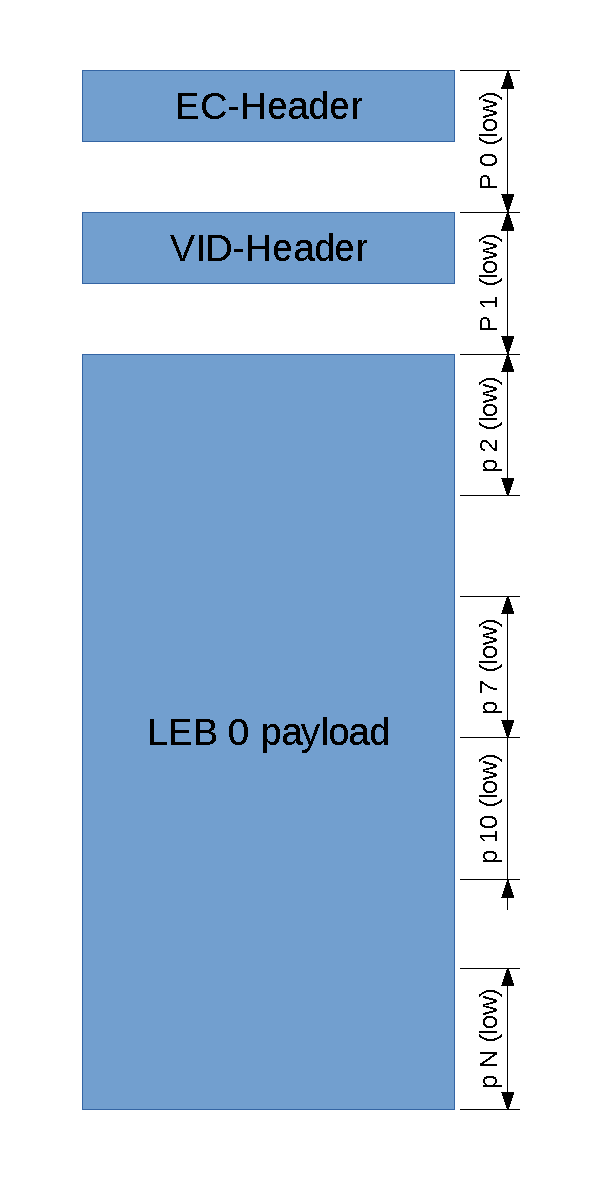
\includegraphics[scale=0.33]{ubi_mlc_slcmode.pdf}
     \end{figure}
   \column{0.7\textwidth}
    \begin{itemize}
    \item MLC does not support subpages.
    \item Only low pages are used, because writes to high pages are more
	  likely to damage data.
    \item Page 0 hosts erase count header.
    \item The next page, page 1 in this example, the volume ID header.
    \item All remaining pages are used for payload.
    \end{itemize}
   \end{columns}
\end{frame}

\begin{frame}[fragile]
\frametitle{UBI PEB in MLC mode on MLC NAND}
   \begin{columns}
   \column{0.3\textwidth}
     \begin{figure}
     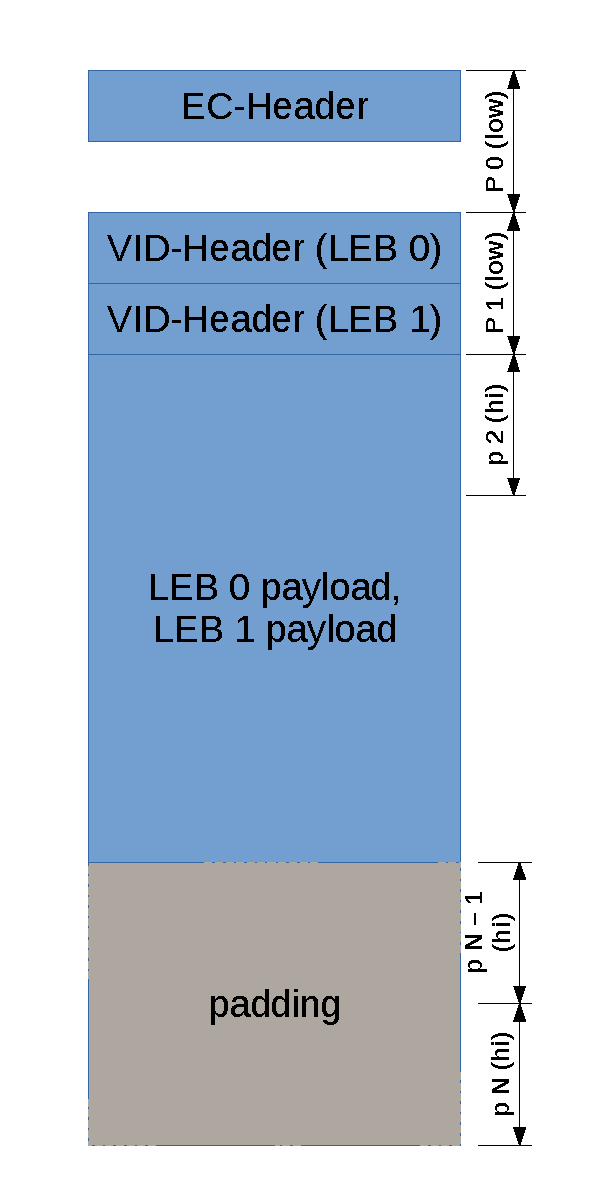
\includegraphics[scale=0.33]{ubi_mlc_conso.pdf}
     \end{figure}
   \column{0.7\textwidth}
    \begin{itemize}
    \item Second page hosts two volume ID headers, one for each LEB payload.
    \item Both low and high pages are used.
    \item Stored data is immutable.
    \end{itemize}
   \end{columns}
\end{frame}

\begin{frame}{Time for some hard-hitting details}
  \begin{itemize}
  \item SLC NAND: 1:1 mapping between PEBs and LEBs.
  \item MLC NAND: 1:2 mapping between PEBs and LEBS.
  \item The LEB and PEB concepts are sometime inter-mixed in UBI, leading
	to confusion with the 1:2 mapping.
  \item Space reservation logic is acting at the PEB level.
  \item Leads to \code{-ENOSPC} if we consider \code{nLEBS = nPEBS x 2}
  \end{itemize}
\end{frame}

\begin{frame}{Fancy new corner cases}
  \begin{itemize}
  \item Consolidated LEBs are immutable.
  \item Consider PEB $x$ in 'SLC mode', it hosts LEB $a$ and UBIFS unmaps LEB $a$.
  \item Since PEB erasure is asynchronous it may take some time until PEB $x$ is erased.
  \item If a power-cut happens we might boot again with LEB $a$ present or not.
  \item UBIFS can deal with that because it keeps track of the usage of all LEBs.
  \end{itemize}
\end{frame}

\begin{frame}{Fancy new corner cases (cont'd)}
  \begin{itemize}
  \item With immutable LEBs a new corner case emerged.
  \item Consider PEB $x$ in 'MLC mode', it hosts LEB $a$ and LEB $b$ and unmaps LEB $a$.
  \item UBI is now not allowed to erase PEB $x$ since LEB $b$ might be still in use, therfore LEB $a$ is marked
        as invalid, in memory.
  \item Now UBIFS allocates LEB $a$ again and writes data to it. After some time it unmaps LEB $a$ again and
        a power-cut happens.
  \item If we are unlucky, PEB $x$ is still present and UBIFS will see the outdated version of LEB $a$ as the most current one.
  \item The solution is that UBIFS must not unmap LEBs which it will allocate later again.
  \item So, we had to change some unmap operations to atomic LEB change operations.
  \item TODO: Last 2 slides would be clearer with a figure!!
  \end{itemize}
\end{frame}

\subsection{Conclusions}

\begin{frame}{Finally, how to use UBI (and UBIFS) on MLC NAND?}
  \begin{itemize}
  \item Teach MTD to know your NAND, especially the pairing.
  \item Also make sure you have strong ECC.
  \item When using ubinize, pass the type of the pairing scheme to it.
  \item Run ubihealthd.
  \end{itemize}
\end{frame}

\begin{frame}{Lessons learned}
  \begin{itemize}
  \item LEB consolidation is slow and source of contentions.
  \item Space reservation is not simple.
  \item LEB and PEB concepts have to be clarified/split.
  \item Long story short, we have a working PoC but it still needs work.
  \item We are working on a second version addressing these aspects:
    \begin{itemize}
    \item Relax locking and work with page chunks when consolidating LEBs.
    \item Fix PEB reservation by moving consolidation at the volume level.
    \end{itemize}
  \end{itemize}
\end{frame}

\begin{frame}[fragile]
\frametitle{V2 plans: How to make consolidation less invasive}
   \begin{columns}
   \column{0.3\textwidth}
     \begin{figure}
     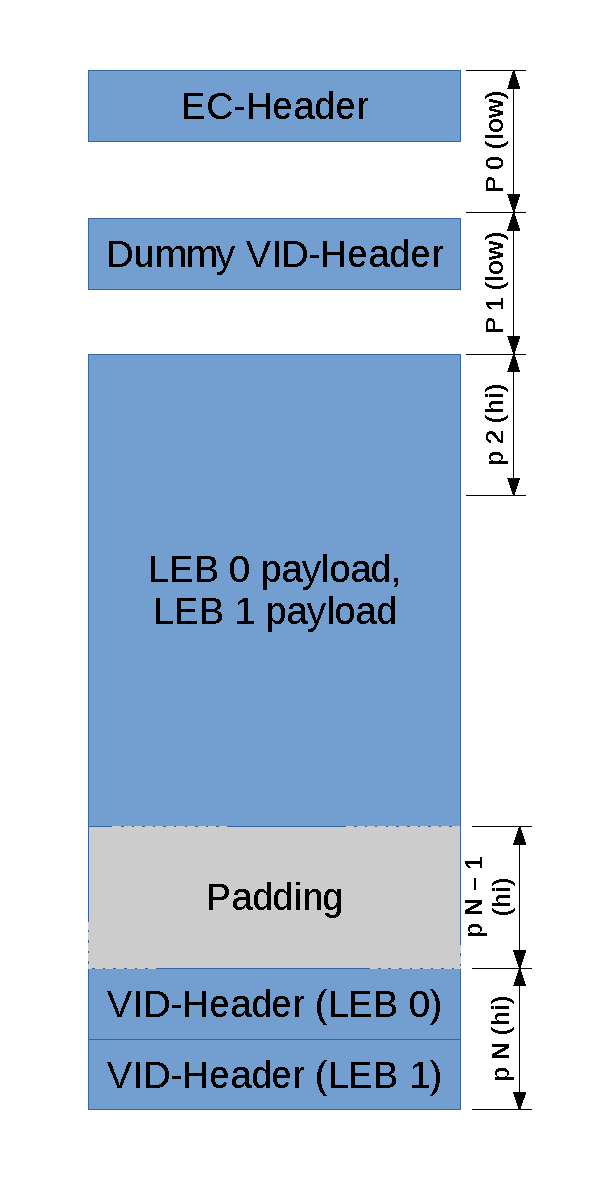
\includegraphics[scale=0.33]{ubi_mlc_conso_dummy.pdf}
     \end{figure}
   \column{0.7\textwidth}
    \begin{itemize}
    \item We use the VID headers as end marker.
    \item If present and valid we can assume that the write process was not interrupted.
    \item No need to compute a checksum of all data.
    \item UBI attach will be faster.
    \end{itemize}
   \end{columns}
\end{frame}

\begin{frame}[fragile]
\frametitle{V2 plans: How to fix LEB/PEB reservation}
   \begin{columns}
   \column{0.3\textwidth}
   \column{0.7\textwidth}
    \begin{itemize}
    \item TODO: add a figure and a description
%  \item One optimization would be placing the VID header at the end of the PEB,
%        that way interrupted writes can be detected by checking only the header and
%        not the CRC of the whole LEB.
%  \item With the current free space accounting model LEB consolidation can still run out of
%        space. This needs fixing.
%  \item Currently LEB consolidation covers the whole UBI instance, like wear leveling.
%        We'd like to limit it to volume scope such that free space accounting will be easier
%        to enforce.
    \end{itemize}
   \end{columns}
\end{frame}

\begin{frame}
  \begin{center}
  \Huge
  Questions? Suggestions? Comments?\\
  \vspace{1.5cm}
  \huge
  Boris Brezillon, Richard Weinberger\\
  \large
  \vspace{0.5cm}
  \code{boris.brezillon@free-electrons.com, richard@sigma-star.at}
  \vspace{0.5cm}
  \newline Slides under CC-BY-SA 3.0\\
  \scriptsize
  \url{http://free-electrons.com/pub/conferences/2016/elce/brezillon-ubi-mlc/}
  \end{center}
\end{frame}

\end{document}
